\listfiles
% \RequirePackage{rotating}
% \documentclass[format=manuscript]{acmart}
\documentclass[format=manuscript, screen,review=true]{acmart}
%\documentclass[format=acmsmall, screen]{acmart}

% bibliography
% using biblatex isn't very smart because journals are pretty picky. Instead use the default natbib package
% \usepackage[backend=biber,style=trad-abbrv,citecounter=true]{biblatex}
% \addbibresource{References.bib}
%
% \renewcommand{\finentrypunct}{%
  % \addperiod\space
  % (Cited \arabic{citecounter}~time\ifnumequal{\value{citecounter}}{1}{}{s})%
% }

%\setcitestyle{super,sort&compress}
% \citestyle{acmauthoryear}
\usepackage{booktabs} % For formal tables
\usepackage[ruled]{algorithm2e} % For algorithms
\usepackage{subcaption}
\usepackage[printwatermark]{xwatermark}
\usepackage{xcolor}
\usepackage{graphicx}
\usepackage{tikz}
\usepackage{nameref}

% \newsavebox\mybox
% \savebox\mybox{\tikz[color=red,opacity=0.3]\node{1st Round Revisions};}
% \newwatermark*[
  % allpages,
  % angle=45,
  % scale=6,
  % xpos=-35,
  % ypos=30
% ]{\usebox\mybox}

% Metadata Information
\acmJournal{CSUR}
\acmVolume{01}
\acmNumber{01}
\acmArticle{01}
\acmYear{2018}
\acmMonth{01}

%\acmBadgeL[http://ctuning.org/ae/ppopp2016.html]{ae-logo}
% \acmBadgeR[http://ctuning.org/ae/ppopp2016.html]{ae-logo}

% Copyright
% \setcopyright{acmcopyright}
%\setcopyright{acmlicensed}
\setcopyright{rightsretained}
%\setcopyright{usgov}
%\setcopyright{usgovmixed}
%\setcopyright{cagov}
%\setcopyright{cagovmixed}

% DOI
\acmDOI{0000001.0000001}

% some useful shortcut commands
\newcommand{\Pl}{\textbf{Pl}}
\newcommand{\R}{\textbf{R}}
\newcommand{\nisarcomm}[1]{{\color{red} (NRA: #1)}}
\newcommand{\brettcomm}[1]{{\color{blue} (BWI: \textbf{#1})}}
\newcommand{\edit}[1]{{\color{blue} #1}}
\newcommand{\hlr}[1]{{\color{red} #1}}

\received{November 2017}
%% 35 pages with references!!!
% Document starts
\begin{document}
% Title portion
\title{``Dave\ldots I can assure you \ldots that it's going to be all right \ldots''} 
 \titlenote{HAL 9000, \textit{2001 A Space Odyssey}, full quote: ``Just what do you think you're doing, Dave? Dave, I really think I'm entitled to an answer to that question. I know everything hasn't been quite right with me, but I can assure you now, very confidently, that it's going to be all right again.''
 }
 \subtitle{A definition, case for, and survey of algorithmic assurances in human-autonomy trust relationships}
 % \subtitlenote{Subtitle note}
\author{Brett W. Israelsen}
    \orcid{0000-0003-1602-1685}
    \email{brett.israelsen@colorado.edu}
    % \affiliation{%
        % \institution{University of Colorado, Boulder}
        % \department{Department of Computer Science}
        % \city{Boulder}
        % \state{CO}
        % \country{USA}
    % }
    % \affiliation{%
        % \institution{RECUV}
    % }
    % \affiliation{%
        % \institution{C-UAS}
    % }
\author{Nisar R. Ahmed}
\authornote{The corresponding author}
    \email{nisar.ahmed@colorado.edu}
    \affiliation{%
        \institution{University of Colorado Boulder}
        % \department{Ann and H.J. Smead Aerospace Engineering Sciences}
        \city{Boulder}
        \state{CO}
        \country{USA}
    }
    \affiliation{%
        \institution{\href{https://cohrint.info/}{Cooperative Human-Robot Intelligence  Laboratory (COHRINT)}}
    }
    \affiliation{%
        \institution{\href{http://www.colorado.edu/recuv/}{Research and Engineering Center for Unmanned Vehicles (RECUV)}}
    }
    %CUAS affiliation is not needed/considered
    %\affiliation{%
    %    \institution{\href{https://c-uas.org/}{Center for Unmanned Aircraft Systems (C-UAS)}}
    %}

\begin{abstract}
    With the advent of artificially intelligent autonomous systems, those who design, use and are otherwise affected by this technology want to know that it will perform correctly, and understand why it does what it does, and how to use it appropriately. That is, they want to be able to \emph{trust} such systems. This work provides a survey of \emph{algorithmic assurances} that allow users to calibrate their trust. Trust between humans and autonomy is reviewed, and the implications for the design of assurances are highlighted \nisarcomm{--todo: revise...this makes the goal of the paper unclear.} A survey of existing research related to algorithmic assurances is presented. Much of the surveyed research originates from fields such as interpretable, comprehensible, transparent, and explainable machine learning, as well as human-computer interaction, human-robot interaction, and e-commerce. Several key ideas are extracted from this work in order to refine the definition of assurances. The design of assurances is found to be highly dependent not only on the capabilities of the autonomous system, but on the characteristics of the human user, and the appropriate trust-related behaviors. Several directions for future research are identified and discussed. \nisarcomm{need to polish this up later...feels like a lot of words that describes details, but that aren't getting at the real core arguments of the paper...}
\end{abstract}

\begin{CCSXML}
<ccs2012>
<concept>
<concept_id>10003120</concept_id>
<concept_desc>Human-centered computing</concept_desc>
<concept_significance>500</concept_significance>
</concept>
<concept>
<concept_id>10010147.10010178</concept_id>
<concept_desc>Computing methodologies~Artificial intelligence</concept_desc>
<concept_significance>500</concept_significance>
</concept>
<concept>
<concept_id>10010147.10010257</concept_id>
<concept_desc>Computing methodologies~Machine learning</concept_desc>
<concept_significance>500</concept_significance>
</concept>
<concept>
<concept_id>10010147.10010341.10010342</concept_id>
<concept_desc>Computing methodologies~Model development and analysis</concept_desc>
<concept_significance>500</concept_significance>
</concept>
<concept>
<concept_id>10010405</concept_id>
<concept_desc>Applied computing</concept_desc>
<concept_significance>500</concept_significance>
</concept>
<concept>
<concept_id>10002978.10003029</concept_id>
<concept_desc>Security and privacy~Human and societal aspects of security and privacy</concept_desc>
<concept_significance>300</concept_significance>
</concept>
</ccs2012>
\end{CCSXML}

% \ccsdesc[500]{Human-centered computing}
% \ccsdesc[500]{Computing methodologies~Artificial intelligence}
% \ccsdesc[500]{Computing methodologies~Machine learning}
% \ccsdesc[500]{Computing methodologies~Model development and analysis}
% \ccsdesc[500]{Applied computing}
% \ccsdesc[300]{Security and privacy~Human and societal aspects of security and privacy}

% We no longer use \terms command
% \terms{Algorithms, Assurances, Trust}

\keywords{human-computer trust, interpretable machine learning, explainable artificial intelligence}

\thanks{This work was funded by a research gift from Northrop-Grumman Aerospace Systems and by the Center for Unmanned Aircraft Systems (C-UAS), a National Science Foundation Industry/University Cooperative Research Center (I/UCRC) under NSF Award No. CNS-1650468 along with significant contributions from C-UAS industry members.}

\maketitle

%%Please keep section headers in this part of the document for easier identification and separability and editing, need to avoid spaghetti code as much as possible.

%%%%%%%%%%%%%%%%%%%%%%%%%%%%%%%%%%%%%%%%%%
\section{Introduction}\label{sec:introduction}
\section{Introduction}
    As technology becomes more advanced, those who design, use, and are affected by it in other ways want to know that it will perform correctly, and understand why it does what is does, and how to use it appropriately. In essence, people who interact with advanced technology want to be able to trust it appropriately, and then act on that trust.

    In interpersonal relationships, and otherwise, humans act largely based on trust. For example, a supervisor asks a subordinate to accomplish a task based on several factors that indicate they can trust them to accomplish that task. When consumers make purchases, they do so with trust that the product will perform as promised. Likewise, when using something like an autonomous vehicle, the user must be able to trust it appropriately in order to use it properly.

    With the rapid advancement of the capabilities of intelligent computing technology to do tasks that were previously assumed to be too complicated for computers, there has been much recent discussion regarding how humans can trust this technology -- although the connection to trust is not always made explicit, per se. This discussion has taken place both in public \cite{Spectrum2016-jv,DeSteno2014-cq,Cranz2017-yh,Cassel2017-tn,Danks2017-sb}, business \cite{Banavar2016-nm, Khosravi2016-ke,Moody2017-vd,Rudnitsky2017-in,Benioff2016-tc}, and academic \cite{Groom2007-bz,Lloyd2014-bb,Goodrum_2016-fm,Foley2017-qj,Ghahramani2015-yq,Castelvecchi2016-mr} settings.

    Those who discuss \emph{how} to trust a specific technology are really referring to the need for some indication of the appropriate level of trust to give said technology. In other words, it is desirable to \emph{design} capabilities and methods for intelligent technology which help us achieve appropriate levels of trust in that technology. These capabilities and methods are collectively referred to as \emph{assurances}. %%
    
    Specifically, this survey investigates what assurances an Artificially Intelligent Agent (AIA) can provide to a human user in order to affect their trust. The colloquial definitions of `appropriate use', `assurance', `AIA', and `trust' should suffice for now to give the reader a general idea of the motivation; more formal definitions will be presented in section \ref{sec:background}. It is the author's position that there are many researchers, from different disciplines, who will potentially be interested in this work. This group includes those who are interested in working with, trusting, interpreting, understanding, and/or regulating AIAs.

    Figure \ref{fig:SimpleTrust_one_way} is a simple diagram of the trust cycle that exists between a human user and an AIA (justification for the existence of this cycle will be presented later). Simply, the user's trust is affected by assurances that in turn affect the user's behaviors in interacting with the AIA (e.g. trust AIA with responsibilities, or not). To fully understand and appreciate the importance of assurances, one must have a more formal understanding of each component in figure \ref{fig:SimpleTrust_one_way}. %This is because the cycle is serial, and cannot be complete with any of the components missing. 
This paper provides an overview of the components of figure \ref{fig:SimpleTrust_one_way}. It then turns a more focused attention to assurances, and investigate some of the research that has been done to date. From this survey of literature, properties and classifications of assurances are created, and directions and considerations for further research are presented.

    \begin{figure}
        \centering
        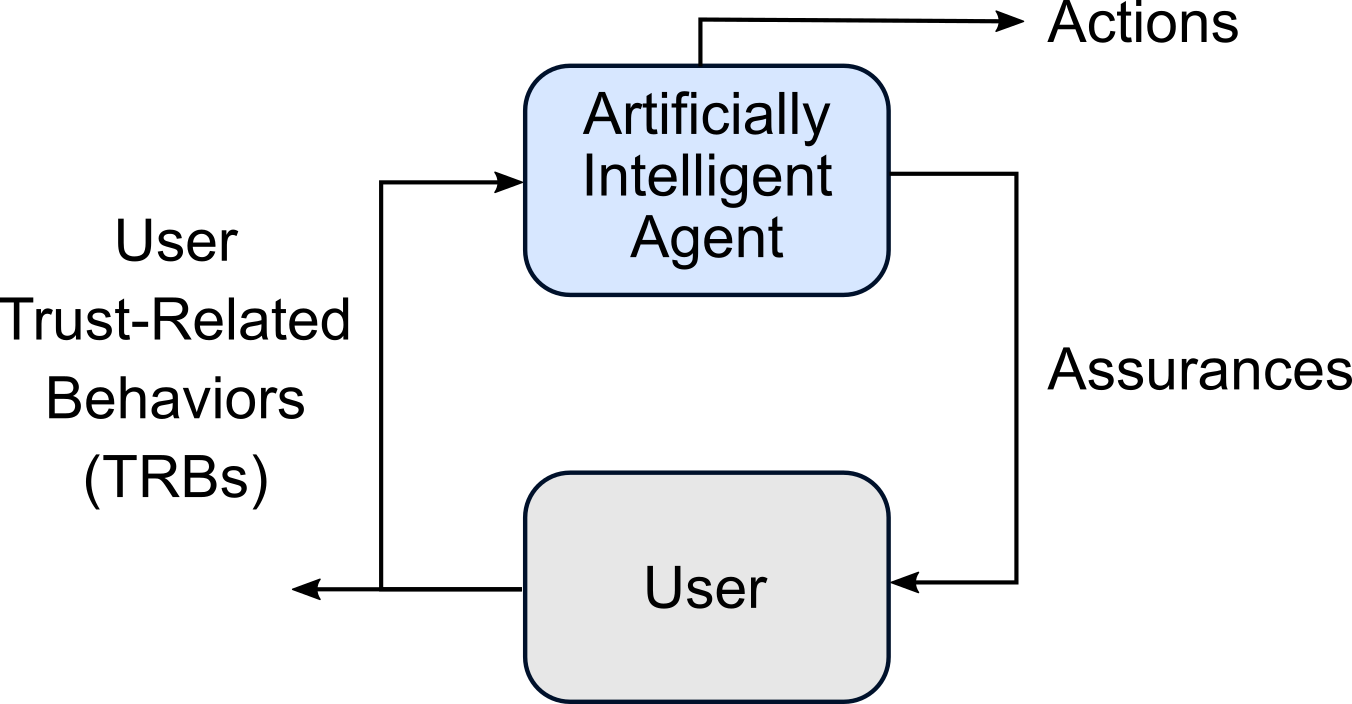
\includegraphics[width=0.7\textwidth]{Figures/SimpleTrust_one_way.png}
        \caption{Diagram depicting the simple one-way trust relationship between a human user and an AIA. Based on a user's level of trust they take certain actions (e.g. give AIA commands), these commands can lead the AIA to certain actions and/or to provide assurances to the user in order to affect their trust.}
        \label{fig:SimpleTrust_one_way}
    \end{figure}

    Some of the novel contributions of this paper include: a detailed description and definition of assurances in general human-AIA relationships; an argument that trust-related behaviors should be used to measure the effect of assurances on user trust; presenting the idea that assurances can be either explicit or implicit; suggestions for promising research directions for explicit assurances.
    % \nisarcomm{This is where the `punchline' and takeaways of this survey should be summarized: i.e. what are the contributions of this work? What are the important arguments to be made? What gaps are being addressed? What is the value of this survey? Who cares about this work? What is interesting/novel about this survey? etc. i.e. what's the point of making the reader read on from here? What's in store for them? Note that this paragraph can be written last, once the remainder of paper is more/less cemented -- but key bullet points should be put in here now/ASAP to build on later}
    To this end, section \ref{sec:background} provides definitions for each of the terms. In section \ref{sec:methodology} I discuss the methodology I used when compiling this survey. Afterwards, section \ref{sec:survey} will discuss the current landscape of assurances that exist in the literature. Finally, section \ref{sec:conclusions} contains some last discussion and conclusions. \nisarcomm{what about Section 5?? -- discuss findings...}


%%%%%%%%%%%%%%%%%%%%%%%%%%%%%%%%%%%%%%%%%%
\section{Motivation and Background} \label{sec:background}
\section{Background and Motivation} \label{sec:background}

\subsection{Motivation}
    Because everyone wants to trust their AIs, whether that be a single classification or regression algorithm, or a more interactive personal assistant that can understand language and communicate. Everyone wants to know how to trust these systems.  

	\begin{sidewaysfigure}[htbp]
        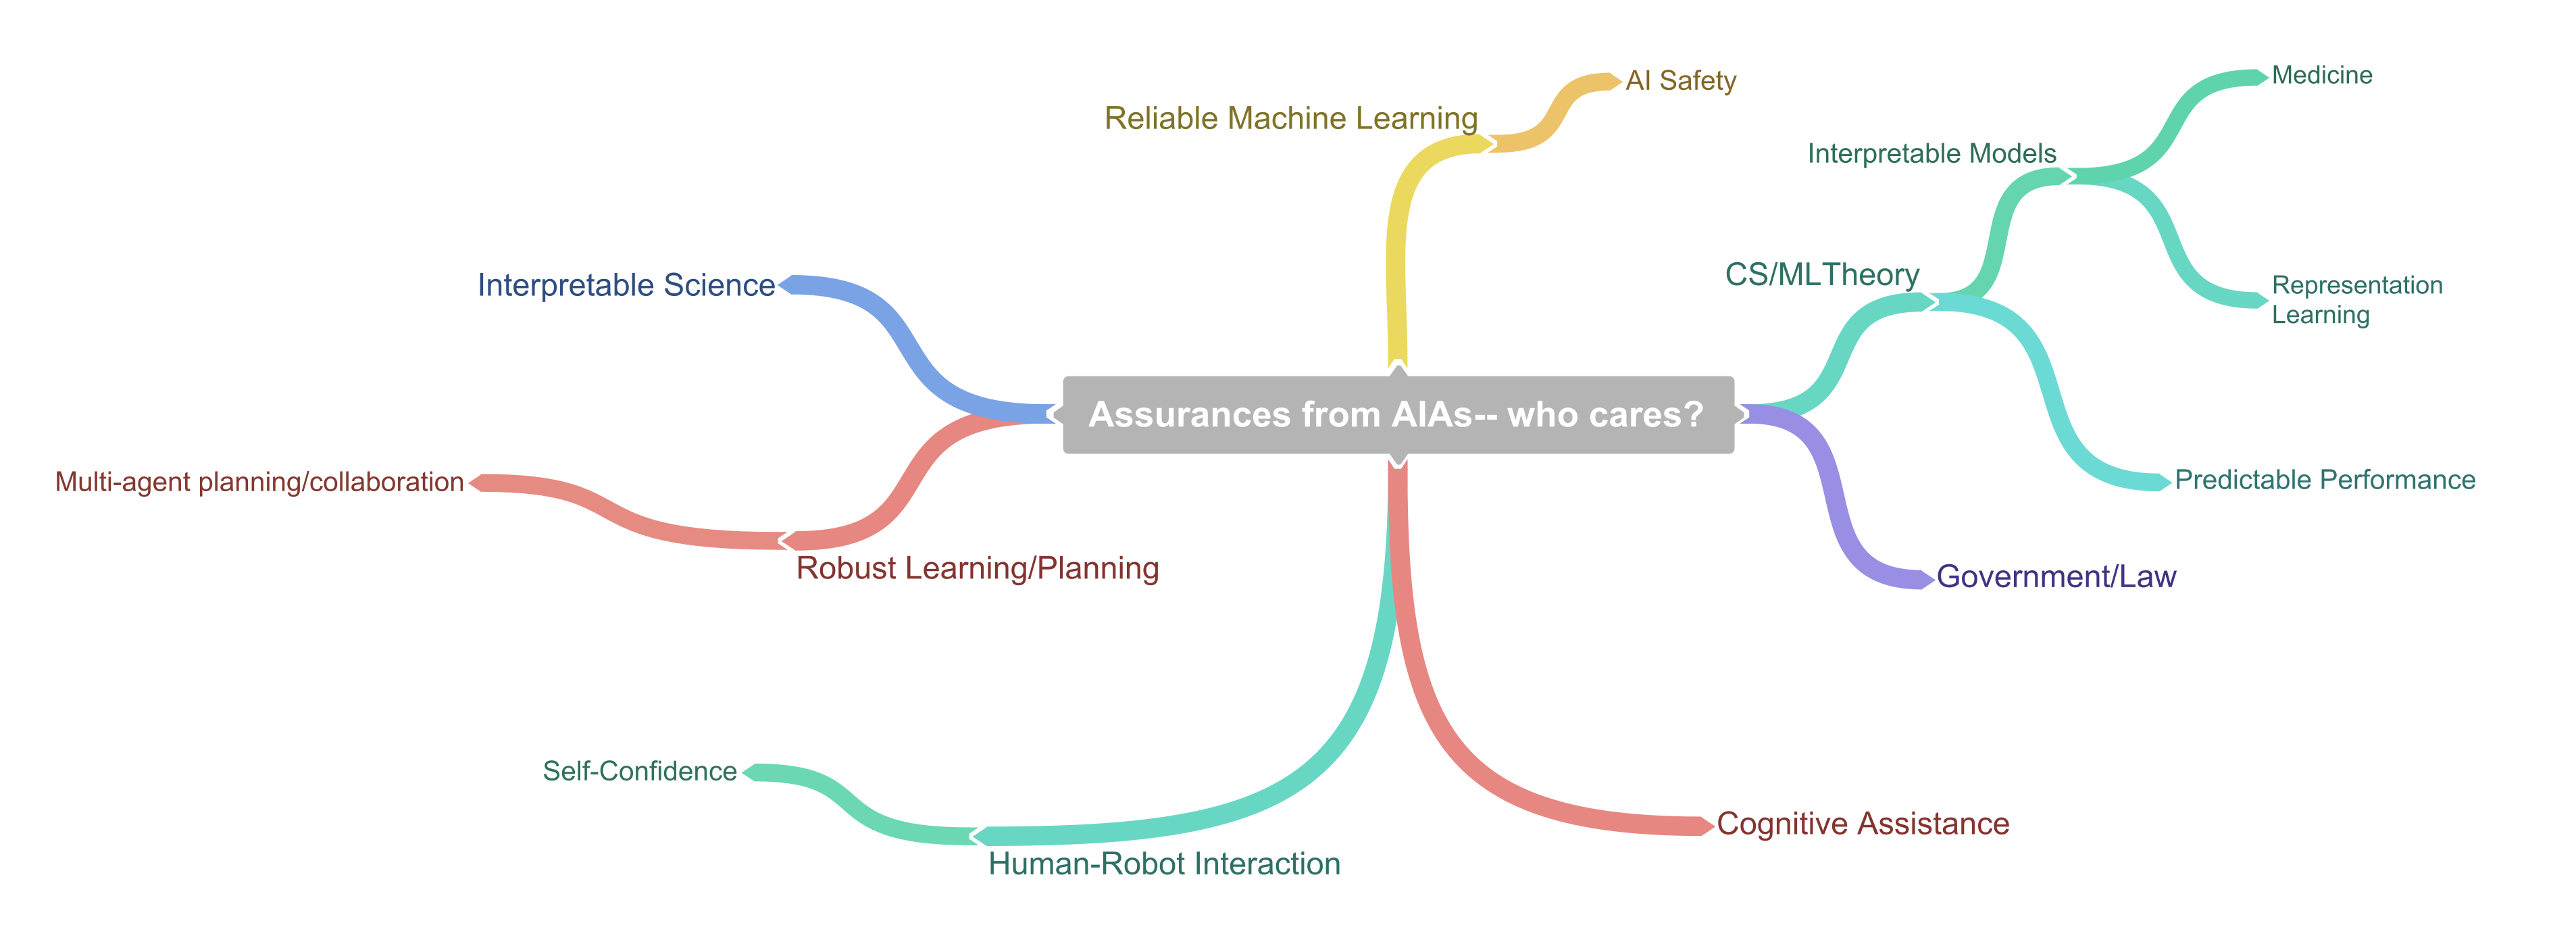
\includegraphics[width=7.5in]{Figures/WhoCares_cleaned}%
    	\caption{A diagram showing some of the academic disciplines that want to trust AIs more fully}
        \label{fig:WhoCares}
    \end{sidewaysfigure}

    \paragraph{Interpretable Science} use data to find causes and insight
    \paragraph{Reliable AI} safety guarantees for robots that have been deployed in real-world environments
    \paragraph{Computer Science} Understand how algorithms will function on real data
    \paragraph{AI/ML} interpret how/why theoretical models function
    \paragraph{Robust Learning/Planning}
    \paragraph{Medicine} understand why data-driven models give predictions
    \paragraph{HCI} help humans and computers interact in a more natural way (where human-human relationships are typically the definition of normal)
    \paragraph{Cognitive Assistance} Ability for user to understand why information was presented
    \paragraph{Government/Law} Regulations on the interpretability of certain algorithms, usage for assistants to lawyers.

    \textbf{Perhaps a table showing the field vs. the AI capability?}, this would help to illustrate the varying needs by fields. Perhaps highlight oversights? \ldots Probably not, we aren't really interested in the different research fields.

\subsection{Artificially Intelligent Agents} \label{sec:aias}
    Intelligent technology spans a wide spectrum of capabilities. With regards to autonomous systems, these might include anything from a thermostat, to the fabled HAL 9000. While the main interest of the authors is geared towards human trust in `advanced' technology, this survey we will take a more holistic view and use the term \textit{Artificially Intelligent Agent (AIA)} to encompass a broad range of technologies that can be considered `autonomous'. This is done in order to provide generally applicable definitions and insights. 

    To this end, an artificially intelligent system needs to possess at least some of the capabilities shown in Figure~\ref{fig:AIcapabilities}~\cite{Russell2010-wv,Nilsson2009-rp,Luger2008-vf}. Some might argue that it is also necessary to add other categories like creativity and social intelligence~\cite{Tao2005-kh}. 
    \brettcomm{SEEMS TO DETRACT---}Some of these categories are also not clearly separable; for instance, where does the capability to `plan' end, and `reasoning' begin? Nevertheless, these capabilities are conceptually useful in defining an AIA:     
    \begin{description}
        \item[Artificially Intelligent Agent (AIA):] an agent that acts on an internally/externally generated goal, and possesses, to some extent, at least one of the capabilities shown in Fig.~\ref{fig:AIcapabilities}.
    \end{description}

	\begin{figure}[htbp]
    	\centering
     	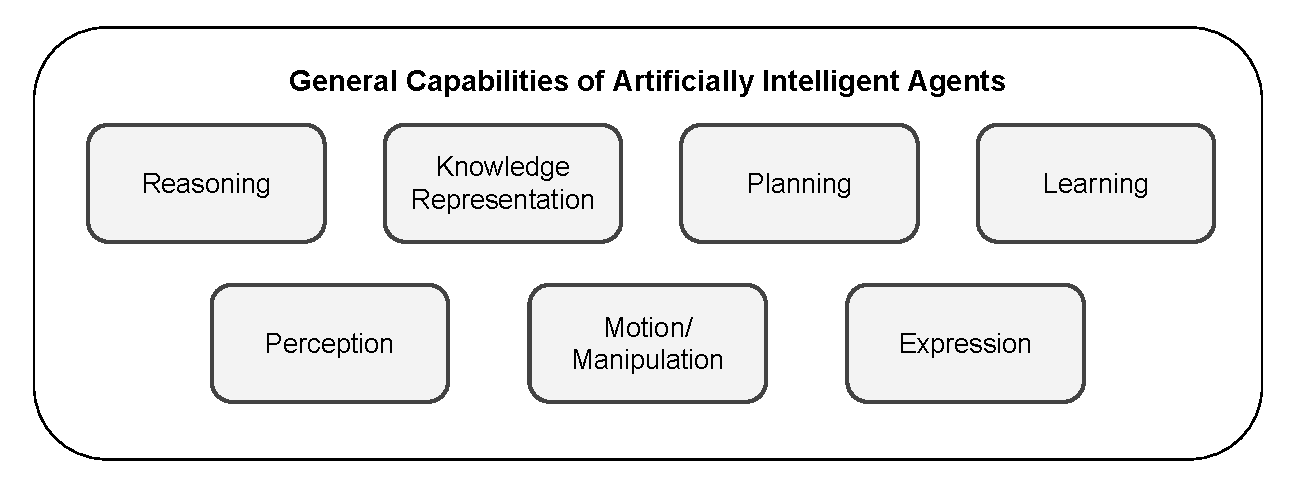
\includegraphics[width=0.55\textwidth]{Figures/AI_capabilities}
    	\caption{List of possible AIA capabilities.}
        \label{fig:AIcapabilities}
    \end{figure}

    The broad range of AIAs implied by this definition is most usefully viewed in terms of scope and adaptability. Scope refers to the range of possible applications for an AIA: does it have a small number of specialized application, or can it be used in many different applications? Adaptability refers to the ability of the AIA to become better at executing its goal over time. Low adaptability has often been associated with `weak AI' whereas high adaptability is often associated with `strong AI'.  Figure~\ref{fig:StrongWeak} depicts these axes for some (real and fictitious) AIAs.

	\begin{figure}[htbp]
    	\centering
     	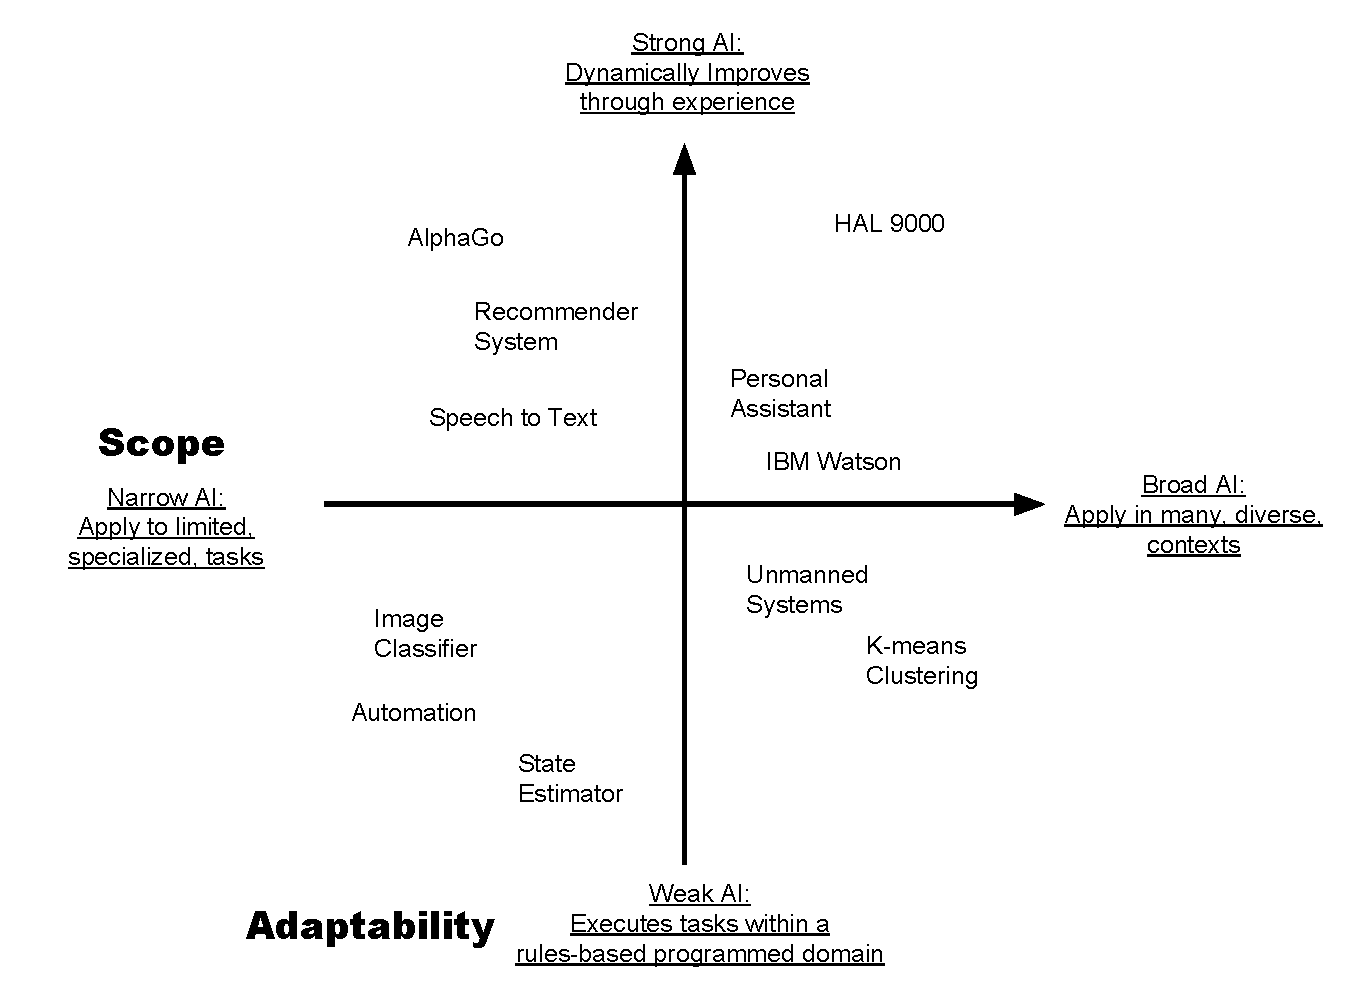
\includegraphics[width=0.7\textwidth]{Figures/strong_weak_narrow_broad.pdf}
    	\caption{Illustration of the range of systems encompassed by the AIA definition. Horizontal axis reflects the scope of the AIA, the vertical axis reflects the adaptability of the AIA.}
        \label{fig:StrongWeak}
    \end{figure}

    Arguably, we might instead have used the term `artificial intelligence' (AI) instead of AIA. However, `AI' carries too much ambiguity (in its fullest meaning, it would possess all capabilities from Figure~\ref{fig:AIcapabilities}, and more). AIA allows the broad inclusion of \emph{any} system in the adaptability/scope plane. The research discipline of machine learning (ML) is a subset of the AI research landscape. Individual ML algorithms might be thought of as being a narrowly scoped AI that is contained within only one of the AIA capabilities. 

    One might also question the need to define AIAs in the first place. This is to aid in the search for and understanding of assurances. As will be shown later, different methods of assurance can be found over the entire range of AIAs, so that an automation system such as a factory robot might be able to use similar assurances -- or more generally, similar principles of assurance -- as might a self-driving car, and vice-versa. The capabilities of AIAs (Fig.~\ref{fig:AIcapabilities}) are the sources of assurances; in other words, assurances cannot exist without some grounding set of AIA capabilities. 

    This definition, while broad, is still useful because it encompasses many of the systems that are typically described as `artificially intelligent'. More importantly, many of the assurances that exist for the simplest AIAs (e.g. chi-square consistency tests for a Kalman filter state estimator) can be adapted/generalized for use in more advanced AIAs. In other words, the proposed definition of AIAs sets an \emph{appropriate scope} for the bodies of research that are likely to have investigated assurances and assurance principles that can be generalized/extended to any intelligent computing system. The definition of AIAs and their range of capabilities also helps to understand and establish what kinds of assurances might be needed in future systems. For example, assurances from an AIA that can only carry out planning tasks will probably differ in design and/or application from assurances from an AIA that can only carry out perception tasks. 

\subsection{User Trust} \label{sec:trust}
    In designing assurances, which affect trust-based user behaviors, it is critical to know what drives those behaviors. Because of this, some time must be spent to understand what trust is. 

    Trust is critical in interpersonal relationships, and it affects the dynamics of \edit{intelligent multi-agent} systems as simple as \edit{one-on-one personal interactions}  \cite{Lewicki2006-hj}, to more complicated ones such as financial markets and governments \cite{Fukuyama1995-un}. Consequently, researchers in psychology, sociology, and economics have historically sought to understand the fundamental principles of trust, each with the aim of understanding their field better \cite{Gambetta1988-pi}. Moral philosophers have also thought intently about the topic \cite{Baier1986-im}.

    Due to wide interest spanning many disciplines it is difficult, if not impossible, to write a succinct definition of trust that would appease all interested parties. Besides that, trust is actually a very broad concept that evades precise definitions at a high level. However the following definition, adapted from \cite{McKnight2004-vv}, is broad enough to avoid too much contention:

    \begin{description}
        \item [Trust:] \edit{a psychological state in which an agent} willingly and securely becomes vulnerable, or depends on, a trustee (e.g., another person, institution, or an AIA), having taken into consideration the characteristics (e.g., benevolence, integrity, competence) of the trustee.
    \end{description}

    \subsubsection{Trust in AIAs and humans?}
        Trust is generally understood to exist between people. Is it possible for a human to enter into a trusting relationship with an AIA?
        % In their paper regarding important human factors that should be considered when designing autonomous machines \cite{Sheridan1984-kx} are seemingly the first to discuss the idea that trust relationships between humans and autonomous systems are important, and to suggest that humans need some assurance that the ``commands will be carried out properly''. They also mention the idea that ``there needs to be an accurate perception of [the autonomous system's] trustworthiness''. Finally they suggest that ``appropriate criteria for trust need to be studied to develop a theory of trust in supervisory control''.
        % Perhaps motivated by \citeauthor{Sheridan1984-kx}\cite{Sheridan1984-kx}, a few years later \cite{Muir1987-mk}, and later in more detail \cite{Muir1994-ow}, create a psychologically based model of trust that considered the ``component expectations of trust'' of \cite{Barber1983-yc} and the dynamic evolution of trust from \cite{Rempel1985-sg}, to make a framework for studying trust in human-machine relationships.
        % \citet{Muir1996-gt} reported the results of two experimental studies to investigate the validity of her proposed model. She claims that these were the first experiments to explicitly ask "operators to rate their trust in automated equipment", and to see if they could do so under normal operating conditions. She found that operators were able to rate their trust in the automation, and that the level of trust changed based on different performance characteristics of the automated system. In her own words: "These results suggest that operators' subjective ratings of trust and the properties of the automation which determine their trust, can be used to predict and optimize the dynamic allocation of functions in automated systems".
        That humans actually do feel trust towards machines has been experimentally confirmed several times in research using common subjective psychological questionnaires. Some examples include: \citet{Muir1996-gt,Reeves1997-ad,Groom2007-bz,Mcknight2011-gv,Riley1996-qm,Bainbridge2011-pl,Kaniarasu2012-mo,Salem2015-md,Desai2012-rc, Freedy2007-sg, Wang2016-id, Inagaki1998-cl, Kaniarasu2013-ho}. 
\nisarcomm{This next part is worth mentioning:} Several academic experiments have investigated the possibility of trust existing between humans and (according to the terminology of this survey) AIAs. All found that some level of trust can be formed in such relationships. For instance, ref. \citet{Lacher2014-yc} points out that people trust an AIA at different levels. For example, an operator would have different perspectives on trust based on their level of interaction with the AIA. The designer of an AIA would also trust the AIA differently than an end user, due to the differing nature of the trust relationship from one to the other. 
        % \citet{Lankton2008-ct} claims, and finds some support for the idea, that trust in technology is fundamentally different from interpersonal trust between humans. They demonstrate the validity of the hypothesis by using a survey of 427 college students regarding Facebook. However, the authors point out that this study was based on a single set of survey data about facebook, and may not be unbiased or apply to other technologies. Beyond this, it is the author's opinion that the `fundamental differences' they point out are not that divergent from the human-human trust model.

        Ref. \citet{Tripp2011-cq} investigate the variation of trust between humans and different levels of technology. They run experiments with three different levels of technology: Microsoft Access, a recommender system, and Faceobook. They found that `human-like' trust applied more to Facebook, while `system-like' trust applied more to MS Access. They conclude that if the system is `human enough', then a human trust model is appropriate. However, the authors also caution that it is important to check first \nisarcomm{Check what first???}.

        Given this research, we will take the position of presenting a human-human trust model and using it as a basis for human-AIA trust -- with the understanding that the applicability of the model varies with the complexity of the AIA. For example, something in the lower-left quadrant of \ref{fig:StrongWeak} \edit{?????} to the upper-right quadrant. \nisarcomm{CAREFULLY READ ALOUD WHAT YOU ARE WRITING: (i) previous sentence is a sentence fragment, and (ii) also this seems like a very strange thing to say: you are applying a human-human trust model as basis for all human-AIA trust, but then you are immediately disclaiming that it is not really applicable in all AIA cases? Then why bother presenting it?! Are you really trying to say something else here, i.e. some features of the model may be more important than other features depending on where you are on the spectrum of adaptability vs. capability? }

\subsubsection{A Model of Human-AIA Trust}
We now present a model of human-AIA trust, which will cast insights on assurances that will be discussed later. It should be noted that this model is being presented as \emph{one possible model} that can be helpful in understanding assurances -- it is neither the only model nor a perfect model. As research advances, such models will also likely continue to evolve, and the ideas of assurances will naturally evolve as well.
        % This has been recently attempted in the context of human-AIA relationships \cite{Lahijanian2016-nd}, but with an overly simplistic reduction of trust. The reality is that trust is extremely complex, and so dealing with it in the setting of human-AIA relationships is going to be complex.

In work relating to business management, McKnight in ref. \citet{McKnight1998-ty} and later in ref. \cite{McKnight2001-fa} performed what is, arguably, the first multi-disciplinary survey and unification of trust literature, which also condensed it into a single typology. The resulting model is shown, with some minor adaptations, in Figure \ref{fig:UserTrust}.

        \begin{figure}[htbp]
            \centering
            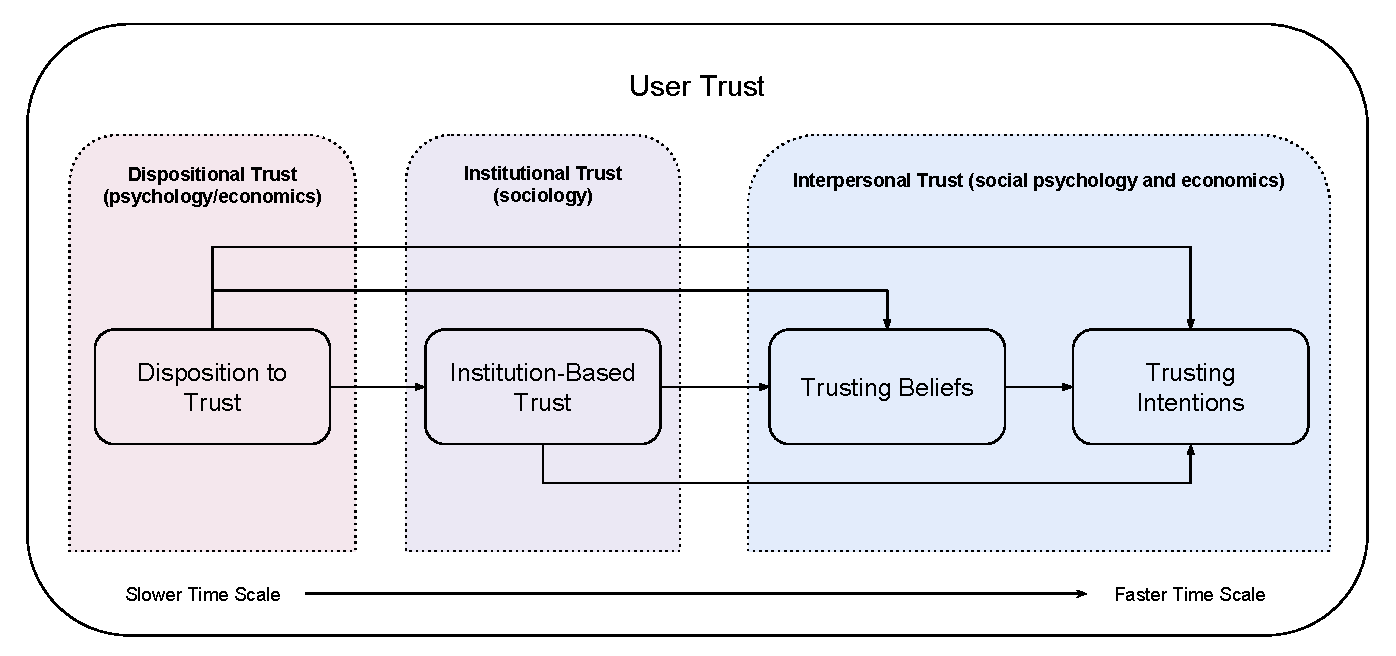
\includegraphics[width=0.9\textwidth]{Figures/UserTrust}
            \caption{Interdisciplinary trust model proposed by \citet{McKnight2001-fa}. The three main categories are delineated, and corresponding disciplines that are interested are listed within parentheses. Connections indicate a causal relationship.}
            \label{fig:UserTrust}
        \end{figure}

        The categories \nisarcomm{of what??} are defined as follows: \nisarcomm{You jumped into the figure without describing anything about it at a high level at all!!! What categories are you talking about -- categories of WHAT exactly??? SAY what the figure means at a high level -- walk the reader through it so they are on the same page as you -- \textbf{DON'T WRITE TO YOURSELF, WRITE FOR YOUR AUDIENCE (WHICH HAS NOT YET SEEN WHAT YOU HAVE SEEN) -- PUT YOURSELF IN AUDIENCE'S SHOES}}

        \begin{description}
            \item [Disposition to Trust:] The extent to which one displays a consistent tendency to be willing to depend on others (and AIA) in general across a broad spectrum of situations and persons
            \item [Institution-Based Trust:] One believes that regulations are in place that are conducive to situational success in an endeavor
            \item [Trusting Beliefs:] One believes that the AIA has one or more characteristics beneficial to oneself
            \item [Trusting Intentions:] One is willing to depend on, or intends to depend on, the AIA even though one cannot control its every action
        \end{description}

        Each of these main categories \edit{of trust} has components defined in Figure \ref{fig:Assurance_classes}. These components were defined through the compilation of many research studies across research disciplines, and because of this represent the most accurate notion of the components of trust available. \edit{It is asserted here} that these trust components \hlr{describe the possible dimensions that constitute trust-related behaviors} \nisarcomm{this is not worded correctly -- these are components of trust, not trust-related behaviors -- they might inform TRBs, but they are not in and of themselves things that constitute TRBs (which you have yet to define at this point!)}, and at which assurances \hlr{must be} targeted. \nisarcomm{MUST be targeted? or are targeted? i.e. is there any real choice? }

        \begin{sidewaysfigure}[htbp]
            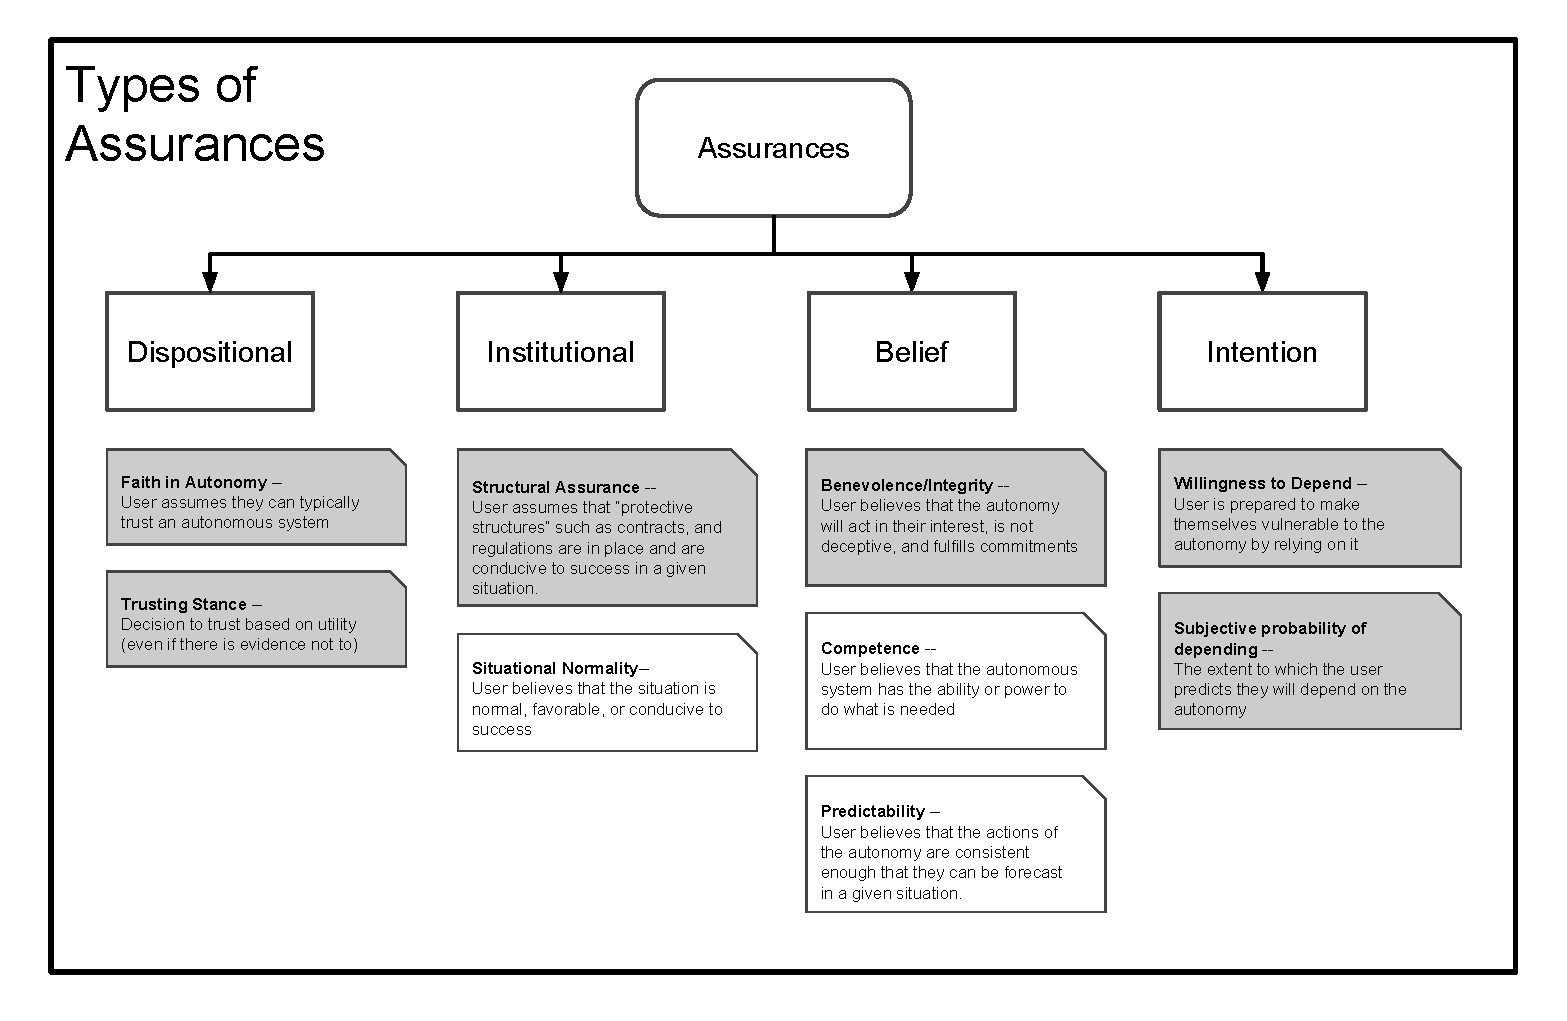
\includegraphics[width=8in]{Figures/Assurances.pdf}%
            \caption{\textbf{Diagram delineating the possible classes of assurances, and suggesting those classes that directly apply in calibration of TRBs \ldots obviously needs to be finished \ldots}}
            \label{fig:Assurance_classes}
        \end{sidewaysfigure}

%trbs.tex
%\nisarcomm{trim, merge, move earlier?....}

%Researchers of all disciplines widely accept that 
Trust ultimately leads to some kind of meaningful behavior or action which reflects the level of trust \cite{Lewis1985-pr}. 
%; this idea was highlighted by \citet{Lewis1985-pr}.  
These are called `trust-related behaviors' (TRBs) \cite{McKnight2001-fa}. %, which is the term that will be used in this survey. 
In the case of a human-AIA relationship per Fig. \ref{fig:SimpleTrust_one_way}, %and \ref{fig:RoadNet}, 
Some example TRBs could include the kinds of tasks the human user assigns to the AIA, accepting and following through on a plan produced by the AIA, or directing that a new plan be made, or switching off autonomous capabilities altogether to teleoperate and perform tasks manually through a physical mechanism that the AIA otherwise controls.  %the vehicle. 

%\subsubsection{Calibration of Trust-Related Behaviors}
    
    Trust is not a univariate quantity that can be objectively measured. Rather, it is a multidimensional phenomenon whose `relative magnitudes and directions' must be observed through changes in TRBs, or qualitative self-reports reported in surveys \cite{Muir1996-gt}. It thus comes as no surprise that TRBs are the more objective measure due to the fact that people are not always consistent in their ratings, and may sincerely feel different levels of trust while performing similar TRBs. \citet{Parasuraman1997-co} were interested in understanding the use of automation by humans, and defined terms to describe that use. Here it is proposed that, by extension, those terms also apply to the behaviors of humans towards more advanced AIAs. Within this scope the definitions are as follows: \textit{Misuse:} over-reliance on an AIA (which could manifest itself in a user's unrealistically optimistic expectations of performance); \textit{Disuse:} under-utilization of an AIA (e.g. a user turning off the AIA, or failing to use all of its capabilities); \textit{Abuse:} Inappropriate application of an AIA (where \emph{application} in this case means the choice to deploy an AIA in a certain context).

    \nisarcomm{can trim down this parag a bit...}
    Following Fig.~\ref{fig:SimpleTrust_one_way}, an AIA's assurances are ideally designed to steer the user away from misuse, disuse, or abuse of the AIA, i.e. towards otherwise appropriate TRBs. This can only be done by properly `calibrating' assurances to suitably influence user trust. This is a point that, to some extent, has been informally mentioned in \cite{Muir1994-ow,Lillard2016-yg,Lee2004-pv,Hutchins2015-if}. Note that other researchers who propose `calibration' (or other similar concepts) often suggest calibrating \emph{trust} as opposed to TRBs. \citet{Dzindolet2003-ts} found that providing system performance feedback tended to increase user's \textit{self-reported trust}, even though user's resulting TRBs did not reflect self-reported trust levels. This shows the danger of calibrating `trust', as opposed to calibrating the TRBs. 
    TRB calibration focuses on concrete and measurable behaviors that are universally applicable. 
    In contrast, trust calibration involves influencing a quantity that is directly immeasurable, and that, when measured indirectly, is subject to individual human differences and biases. 
\subsection{Assurances} \ref{sec:assurances}
    The term assurances was introduced in the previous section as the name by which feedback will be known in a human-AIA trust relationship. As assurances are the main topic of this paper, and are have received very little attention in trust literature, a more detailed definition and discussion is merited.

    \citet{McKnight2001-fa} allude to this kind of feedback in an e-commerce relationship as `Web Vendor Interventions' and mention some possible actions that might be used in that specific application. They go as far as making a diagram that indicates that these interventions could affect the `Trusting Beliefs', `Trusting Intentions', and `Trust-Related Behaviors' (see Figure \ref{fig:UserTrust}).

    \citet{Corritore2003-gx} refer to assurances as `trust cues' that can influence how online users trust vendors in an e-commerce setting. \citet{Lee2004-pv} discuss `display characteristics', which are methods by which an autonomous can communicate information to an operator.
    
    The term assurances is perhaps earliest used in the context of human-automation relationships by \citet{Sheridan1984-kx}. More recently, and formally, \citet{Lillard2016-yg} defined the term `assurance', I extend the definition to be more general
    
    \begin{description}
        \item [Assurance:] A property or behavior of an AIA that affects a user's trust. As used here, the term is not intended to have a positive or negative connotation -- assurances can decrease trust.
    \end{description}

    Most familiar with the fields of AI, ML, data science, and robotics will recognize terms like \emph{interpretable}, \emph{comprehensible}, \emph{transparent}, \emph{verified and validated}, \emph{certified}, and \emph{explainable AI}, with respect to the models or performance of a designed system. A key claim of this paper is that from a high level all of these terms have the same aim: for a user to be able to trust an AIA to operate in a certain way, and based on that trust behave appropriately towards the AIA. Those actions might include re-design, as well as adjusting TRBs.
%
    % Assurances and `interpretability' are delicately linked. In fact, interpretability would be classified as one embodiment of an assurance. This relationship is highlighted by \citet{Vellido2012-nm} where they illustrate that interpreting an AIA is part of the knowledge discovery process.

    The sections that follow outline different classes of assurances.

    \subsubsection{Source-Target Classification}
    It is convenient to refer to assurances by way of their source and target. Intuitively, there may be a set of different algorithms that are useful for making assurances that convey information about planning to the competence dimension of the user's trust. It is easier to refer to these assurances in terms of their source and target. So, for this example that class of algorithms would be the `planning-competence' class.
    
    Not only is this useful shorthand for communicating about the purpose of the algorithms, but it is useful in classifying the range of assurance algorithms that exist. There may also be a class of algorithms that span multiple source-target capabilities. For example there may be a kind of algorithm that can give a `learning-competence' assurance, as well as a `planning-competence' assurance.

    This is especially true since many of the AIA capabilities can overlap. Also, the effects of assurances cannot be guaranteed to affect only one trust dimension.

    Figure \ref{fig:Assurance_classes} shows the hierarchy of proposed assurance classes. The categories mirror those of the trust model proposed by \citet{McKnight2001-fa}, but with the emphasis on what an AIA has the ability to most readily influence (and consequently where most research is found). The boxes with the beveled corner identify and define the different classes of assurances. All classes are included here for completeness and generality. Although, while it is hypothetically possible for an AIA to influence a persons general `Trusting stance' given enough time\footnote{One might imagine an AIA that specifically speaks to the human about the benefits or drawbacks about trusting even though there might not be evidence to do so, similar to the role a counselor might play}, the gray boxes are not considered further in this survey, as practically no direct research exists in the realm of human-AIA relationships.

    \textbf{ugggg, this gets a little complicated, but it's not supposed to be}.

    \subsection{Component and Composite Assurances}
Assurances can be either component or composite. This was seen a little through the survey. The definitions are as follows:

\begin{description}
    \item [Component:] An assurance that originates from a single AIA capability source, and targets a single trust dimension target.
    \item [Composite:] The combination of more than one component assurance into a single assurance. 
\end{description}

\begin{figure}[!htbp]
    \centering
    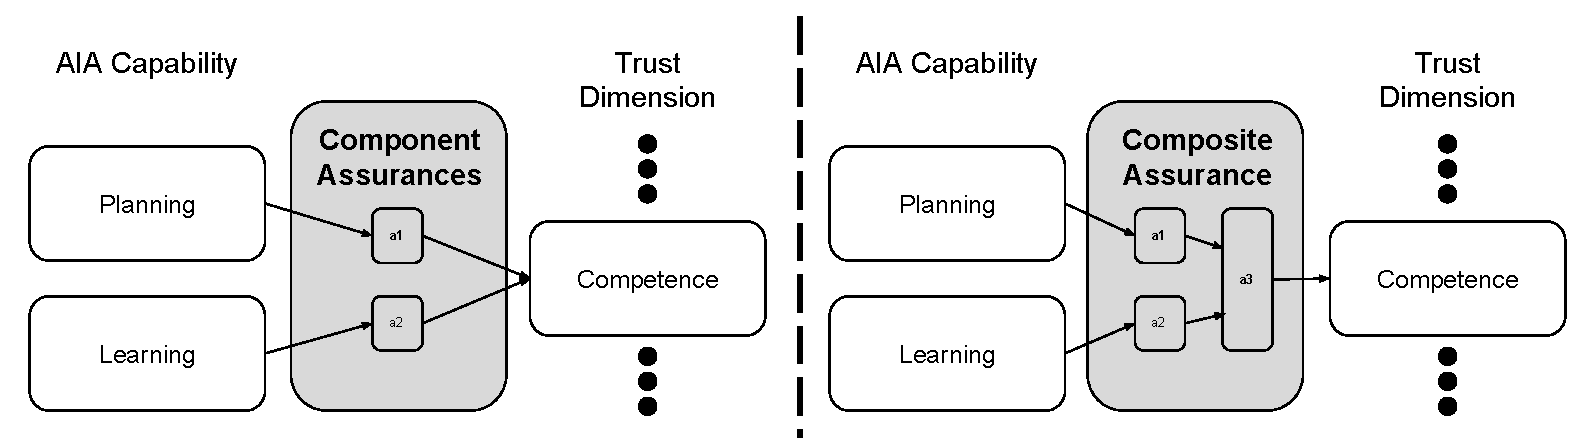
\includegraphics[width=0.9\textwidth]{Figures/Assurance_component_composite.pdf}
    \caption{Figure illustrating the difference between component and composite assurances. The existence of multiple assurances does not imply a composite assurances, rather the combination of multiple component assurances into a single assurance constitutes a composite assurance.}
    \label{fig:assurance_mapping}
\end{figure}

Figure \ref{fig:assurance_mapping} illustrates the concepts of component and composite assurances.

\paragraph{Component Assurances:} Component assurances are perhaps the most well researched in the existing literature. This is likely because several verified component assurances are the predecessors to composite ones. A component assurance might include displaying the confidence of a classification prediction, or visualizing a model as discussed in section \ref{sec:q2}.

\paragraph{Composite Assurances:} Composite assurances are assurances that are built of several components. A notable example is the work by \citet{Aitken2016-cv} who propose a measurement called `self-confidence', applicable to Partially Observable Markov Decision Processes (POMDPs). This metric combines five component assurances into a single composite assurance that is meant to distill the information into a value that a novice operator could understand easily. This paper was discussed in more detail in \ref{sec:q2}. 

    \emph{Tutoring vs Telling:}
Most assurances investigated to date are `telling', in that they do not consider the experience or other traits of different users. The ability to adapt to different users, and to tutor them to appropriate trust will become more critical as time passes due to the diversity of users bases for advanced AIAs and time that users will interact with them. A tutoring assurance would be a planned, dynamic, sequence of assurances that would change in time to adapt to the user's needs. This might include modification of assurances to help a user avoid boredom, or to use the system differently in varying circumstances. It isn't surprising that, to our knowledge, no research has been done with respect to tutoring a user in a trust relationship. This is a complex problem to address that would involve understanding how different users learn, and what an appropriate strategy would be to teach them to have appropriate TRBs. However, a rich resource (not investigated in this paper) would be the work on tutoring systems \citet{Wenger2014-ld} and algorithmic teaching \citet{Balbach2009-jw}.

    \subsubsection{Explicit and Implicit Assurances}
\citet{Sheridan1984-kx} briefly alluded to the existence of explicit and implicit assurances when they discussed the nature of how humans behave when working with automated systems. They suggested that the operator's perception of the automated system can be effected by `performance' and its `reports on its own performance'. 


\begin{description}
    \item [Explicit:] Assurances that are purposefully given to affect the trust of a user.
    \begin{itemize}
        \item Legible motion \cite{Dragan2013-wd}, which is motion calculated with the intent of being more understandable by a human
        \item $R^2$ value, gives some indication of how well the regression accounts for the variance of the data
    \end{itemize}
    \item [Implicit:] All other assurances that aren't explicit.
    \begin{itemize}
        \item Reliability in completing a task. Generally, the object of success is not to affect the user's trust (although this is a nice side-effect).
        \item The way an autonomous vehicle appears. For example something that looks neat will have a different effect on trust, than an AIA with wires dragging on the ground. 
    \end{itemize}
\end{description}




    \subsubsection{The \edit{Imprecise} Nature of Assurances}
        Due to the nature of trust (and humans in general), a single assurance might be targeted at influencing the competence dimension of trust, but it may also have effects on other dimensions. As an example an assurance aimed at influencing Predictability may also have an affect on the Probability of Depending.

        Besides being difficult to separate, each user is different. Thus no assurance will have an identical effect when given to two separate users. This makes it difficult to have precise effects on user trust behaviors.

        \textbf{I am not sure how I want this argument to go, I want to highlight that it is theoretically possible to have some affect on each of these attributes, but that some are more practical. Two main things need to be considred 1) time-scale (how long will it take to make a noticeable change), and 2) what SHOULD be influenced in order to appropriately calibrate TRBs (it probably isn't acceptable to lie in order to manipulate a user's trust)?}



%%%%%%%%%%%%%%%%%%%%%%%%%%%%%%%%%%%%%%%%%%
\section{Survey of Algorithmic Assurances} \label{sec:synthesis}
\section{Survey Sections} \label{sec:survey}
Now that AIA, assurances, trust, and TRBs have been defined we are ready to being the survey regarding what assurances exist, and how to proceed with their design. The obvious place to start is with those researchers who have formally addressed the topic of trust between humans and AIAs of some form. Here we consider formal treatment of trust to be those who acknowledge a human trust model and who perform experiments that attempt to measure the effect of assurances on trust.

However, this leaves out a much larger body of those who have informally considered trust in their work. In this case I define informal to mean those who only reference the nebulous idea of trust, and who do not actually perform experiments to verify that assurances actually do affect trust.

Conversely, much of the formal research has focused on implicit assurances. This is likely due to the focus on analyzing the effect of autonomous systems on trust and not on designing systems for trust. However as seen by a large spike in interest in `interpretable', and `explainable' AIAs in government, academic, and public circles, there is a large need for designed assurances.

\begin{figure}[htbp]
    \centering
    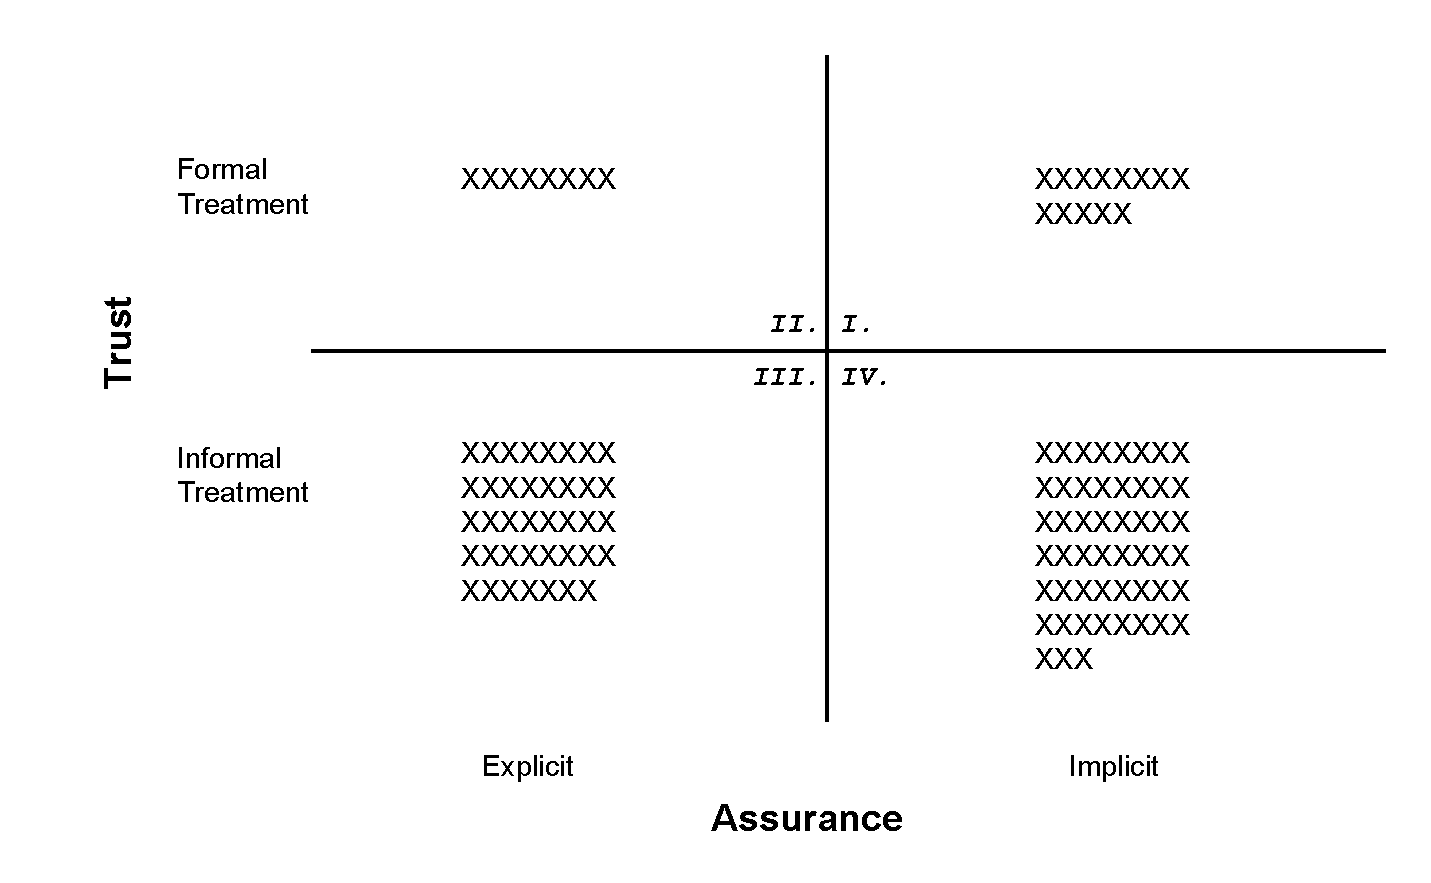
\includegraphics[width=0.6\textwidth]{Figures/Trust_vs_Assurance_Intention.pdf}
    \caption{Figure depicting how many papers that consider trust formally/informally consider intentional/unintentional assurances, \textbf{need to put actual data here, if it is a useful figure, for now the data is approximate from my memory}}
    \label{fig:trust_assurance_intention}
\end{figure}

The remainder of this survey will focus on surveying the assurance research in the formal/informal, explicit/implicit plane. Figure \ref{fig:trust_assurance_intention} shows the number of papers considered in this survey that lay in each quadrant of that plane. The quadrants are defined as:

\begin{itemize}
    \item Quadrant I. (implicit, formal) -- Use human experiments, consider a trust model, assurances are implicit (i.e. those who care about trust, but aren't designing assurance algorithms)
    \item Quadrant II. (explicit, formal) -- Use human experiments, consider a trust model, assurances are explicit (i.e. those who formally acknowledge trust from an AIA, and design assurances to affect it)
    \item Quadrant III. (explicit, informal) -- No human experiments, reference trust (or interpretability, etc..), proposed assurances are explicit (i.e. those who know that ``trust'' is important, but really just present their opinion about an algorithm that might be an assurance)
    \item Quadrant IV. (implicit, informal) -- don't reference trust, designed properties of AIA for better performance, typically reference some of the trust components such as predictability, stability, verification, but only in the context of the designer being happy.(i.e. those whose work is relevant for assurances, but they don't know it)
\end{itemize}

It is clear that much of the research that is relevant has occurred in the informal half of the plane. The aim, in order to satisfy the need for trust in AIAs, is to create more research in Quadrant II. This would mean that assurances have been formally and explicitly designed to affect user's trust. One key observation, is that there is plenty of opportunity to `move' research from Quadrants I., III., and IV. to Quadrant II. In essence this would be taking proposed methods and putting them to the test using a formal understanding of trust and appropriately designed experiments.

\subsection{Intentional and Unintentional Assurances}
    There seems to be quite a large disparity of the kinds of assurances studied by the formal and informal trust groups, as depicted in Figure \ref{fig:trust_assurance_intention}.  This is most likely due to the differing interests and skill sets. Those studying unintentional assurances seem to be more interested in investigating the human-AIA relationship. On the other hand those investigating the effect of intentional assurances are more interested in making algorithms.
    
    This figure clearly shows that there is a large space for researchers who study intentional assurances within a formal trust framework. To state the idea more clearly, this would involve actively designing assurances based on the AIA capability, and the assurance classes, and then validating these assurances in designed experiments.

    \textbf{add more stuff \ldots}


\subsection{Other stuff \ldots}


%%%%%%%%%%%%%%%%%%%%%%%%%%%%%%%%%%%%%%%%%%
\section{Future Work} \label{sec:future_work}
\section{Future Work} \label{sec:future_work}
\brettcomm{Add more stuff about avenues for future work}

\begin{itemize}
    \item Draw from other disciplines that have `useful' tools. (stuff from old Q4)
    \item How to know if assurances are effective. Are explicit assurances being perceived as desired? Are implicit assurances overpowering?
    \item component and composite assurances. What happens when assurances are combined vs. when they exist in isolation? How should assurances be combined?
    \item methods, and modes of expression. What human limitations must be considered
    \item from the perspective of AIAs are there assurances that exist for each of the capabilities that can communicate to the different trust targets?
    \item currently assurances are typically `displayed' as static information to a user, can a user be taught over time by planning assurances?
    \item distrust
    \item two-way trust
\end{itemize}

\subsection{Component and Composite Assurances}
Assurances can be either component or composite. This was seen a little through the survey. The definitions are as follows:

\begin{description}
    \item [Component:] An assurance that originates from a single AIA capability source, and targets a single trust dimension target.
    \item [Composite:] The combination of more than one component assurance into a single assurance. 
\end{description}

\begin{figure}[!htbp]
    \centering
    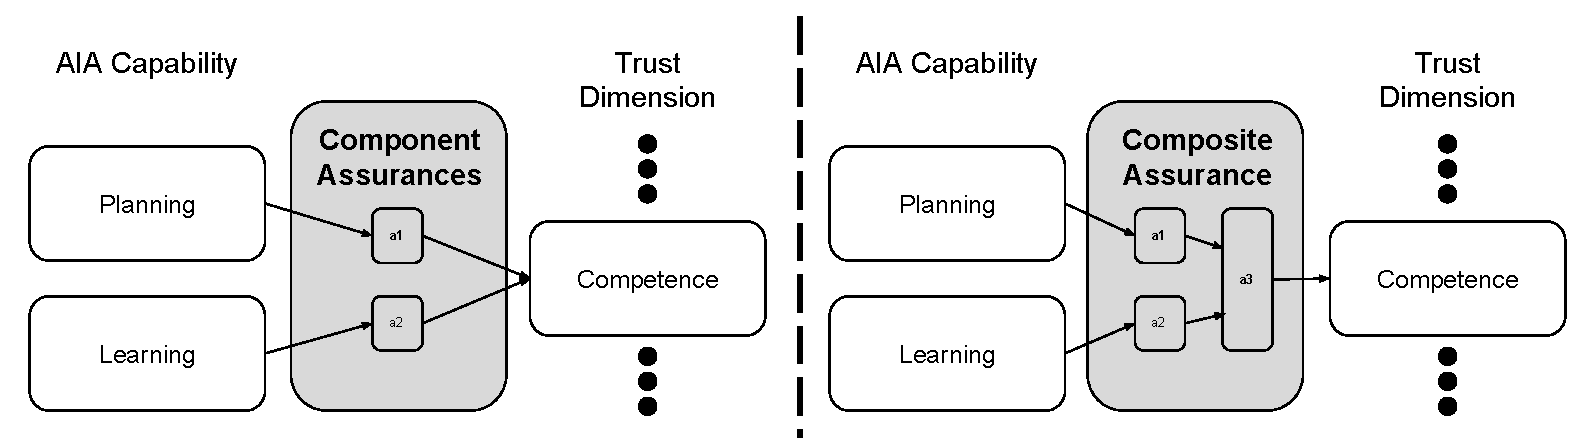
\includegraphics[width=0.9\textwidth]{Figures/Assurance_component_composite.pdf}
    \caption{Figure illustrating the difference between component and composite assurances. The existence of multiple assurances does not imply a composite assurances, rather the combination of multiple component assurances into a single assurance constitutes a composite assurance.}
    \label{fig:assurance_mapping}
\end{figure}

Figure \ref{fig:assurance_mapping} illustrates the concepts of component and composite assurances.

\paragraph{Component Assurances:} Component assurances are perhaps the most well researched in the existing literature. This is likely because several verified component assurances are the predecessors to composite ones. A component assurance might include displaying the confidence of a classification prediction, or visualizing a model as discussed in section \ref{sec:q2}.

\paragraph{Composite Assurances:} Composite assurances are assurances that are built of several components. A notable example is the work by \citet{Aitken2016-cv} who propose a measurement called `self-confidence', applicable to Partially Observable Markov Decision Processes (POMDPs). This metric combines five component assurances into a single composite assurance that is meant to distill the information into a value that a novice operator could understand easily. This paper was discussed in more detail in \ref{sec:q2}. 

\subsubsection{Explicit and Implicit Assurances}
\citet{Sheridan1984-kx} briefly alluded to the existence of explicit and implicit assurances when they discussed the nature of how humans behave when working with automated systems. They suggested that the operator's perception of the automated system can be effected by `performance' and its `reports on its own performance'. 


\begin{description}
    \item [Explicit:] Assurances that are purposefully given to affect the trust of a user.
    \begin{itemize}
        \item Legible motion \cite{Dragan2013-wd}, which is motion calculated with the intent of being more understandable by a human
        \item $R^2$ value, gives some indication of how well the regression accounts for the variance of the data
    \end{itemize}
    \item [Implicit:] All other assurances that aren't explicit.
    \begin{itemize}
        \item Reliability in completing a task. Generally, the object of success is not to affect the user's trust (although this is a nice side-effect).
        \item The way an autonomous vehicle appears. For example something that looks neat will have a different effect on trust, than an AIA with wires dragging on the ground. 
    \end{itemize}
\end{description}



\emph{Tutoring vs Telling:}
Most assurances investigated to date are `telling', in that they do not consider the experience or other traits of different users. The ability to adapt to different users, and to tutor them to appropriate trust will become more critical as time passes due to the diversity of users bases for advanced AIAs and time that users will interact with them. A tutoring assurance would be a planned, dynamic, sequence of assurances that would change in time to adapt to the user's needs. This might include modification of assurances to help a user avoid boredom, or to use the system differently in varying circumstances. It isn't surprising that, to our knowledge, no research has been done with respect to tutoring a user in a trust relationship. This is a complex problem to address that would involve understanding how different users learn, and what an appropriate strategy would be to teach them to have appropriate TRBs. However, a rich resource (not investigated in this paper) would be the work on tutoring systems \citet{Wenger2014-ld} and algorithmic teaching \citet{Balbach2009-jw}.

\subsubsection{Source-Target Classification}
    It is convenient to refer to assurances by way of their source and target. Intuitively, there may be a set of different algorithms that are useful for making assurances that convey information about planning to the competence dimension of the user's trust. It is easier to refer to these assurances in terms of their source and target. So, for this example that class of algorithms would be the `planning-competence' class.
    
    Not only is this useful shorthand for communicating about the purpose of the algorithms, but it is useful in classifying the range of assurance algorithms that exist. There may also be a class of algorithms that span multiple source-target capabilities. For example there may be a kind of algorithm that can give a `learning-competence' assurance, as well as a `planning-competence' assurance.

    This is especially true since many of the AIA capabilities can overlap. Also, the effects of assurances cannot be guaranteed to affect only one trust dimension.

    Figure \ref{fig:Assurance_classes} shows the hierarchy of proposed assurance classes. The categories mirror those of the trust model proposed by \citet{McKnight2001-fa}, but with the emphasis on what an AIA has the ability to most readily influence (and consequently where most research is found). The boxes with the beveled corner identify and define the different classes of assurances. All classes are included here for completeness and generality. Although, while it is hypothetically possible for an AIA to influence a persons general `Trusting stance' given enough time\footnote{One might imagine an AIA that specifically speaks to the human about the benefits or drawbacks about trusting even though there might not be evidence to do so, similar to the role a counselor might play}, the gray boxes are not considered further in this survey, as practically no direct research exists in the realm of human-AIA relationships.

    \textbf{ugggg, this gets a little complicated, but it's not supposed to be}.


\subsection{Distrust}
The treatment of assurances in this survey is based, in part, on a model of interpersonal trust. For completeness it is important to mention the concept of \textit{distrust}, as reviewed and discussed by \citet{Lewicki1998-ox}, and formalized in \citet{McKnight2001-gz}. Low trust is not the same as distrust, and low distrust is not the same as trust. \citet{McKnight2001-gz} suggest that ``the emotional intensity of distrust distinguishes it from trust'', and they explain that distrust comes from emotions like: wariness, caution, and fear. Whereas, trust stems from emotions like: hope, safety, and confidence. Trust and distrust are orthogonal elements that define a person's TRB towards a trustee. In this survey, distrust was not considered. However it must be made clear that any \emph{complete} treatment of trust relationships, and for our purposes, designed assurances, must consider the dimensions of distrust as well as those of trust. For now, this is left as an avenue for future research (one yet to be picked up by mainstream AIA researchers).

\subsection{Expression and Perception of Assurances} \label{sec:express_assurances}
Although specific algorithms can be used to build the contents of assurances, it is also critical to consider the actual communication of assurances. The expression (and subsequent perception) of an assurance involves considering mediums, methods, and efficacy. The medium of an assurance includes the form in which it expressed, e.g. visually, audibly, or otherwise. 
The method of expression includes for example using a plot, or a natural language phrase (which could be text-based or speech-based, depending on the medium).  Finally, the factors influencing the efficacy of the assurance must also be considered (e.g. consider using an audible assurance in a noisy environment). Humans generally utilize different methods/mediums when communicating assurances to each other to maintain efficacy when potential `losses in transfer' might occur. 
However, arguably the greatest challenge in using different mediums and methods is not in their implementation, but in designing the ability to recognize and decide when they should be applied. Some interesting questions are: In what circumstances are different methods most useful? And the same for mediums? How can different methods/mediums be selected in order to maximize assurance efficacy while also taking into account that using all possible combinations will \emph{not} help the user? How, and to what extent, can AIAs assess the efficacy of an assurance before, during, or after operation?

\subsection{Observing Effects of Assurances} \label{sec:measuring_effects}
    Since assurances are meant to influence TRBs, it is important to quantify those effects so that:  1) the AIA system designer can understand how effective the assurances are; and 2) the AIA can observe and respond to/adjust the efficacy of its assurances. To our knowledge, there has not been any work that enables an AIA to observe user responses to assurances and then adapt behaviors appropriately (at least not in the trust cycle setting). 
    Yet, this capability is crucial for enabling AIAs to meet different user's needs. 
Theoretically, any method that is made for the designer to measure the effects of assurances could also be deployed by the AIA itself to assess the effects of assurances on user TRBs. 
The surveyed literature gives some insights into how that has been done to date; namely, there are two main approaches: (1)  Gather self-reported changes in trust from human users; and (2) Measure changes in user's TRBs. 
    
\subsubsection{Self-Reported Changes in Trust} Assessing self-reported changes in trust involves asking users to answer questions, such as `how trustworthy do you feel the system is?'; or `to what extent do you find the system to be interpretable?', either while using a system or afterwards \cite{Mcknight2011-gv,Muir1996-gt,Wickens1999-la,Salem2015-md,Kaniarasu2013-ho}. These kinds of questions are useful in verifying whether the assurances are having the expected effects. It is not unreasonable to imagine that an AIA might be equipped to ask users questions about their trust, process those responses, and modify assurances appropriately.

Self-reports are the most useful when trying to understand the true effects of an assurance. Does a certain assurance, assumed to affect `situational normality', actually do that? 
Does displaying a specific plot actually convey information about `predictability'? 
There is much room for research in this area, which can be used to inform the selection of the methods of assurance. 
However, changes in self-reported trust do not always result in changes in TRBs \cite{Dzindolet2003-ts}. From the AIAs perspective this means that --- unless the object of the assurances is to make the person's level of self-reported trust change --- the assurances may not be providing any tangible benefit. 
As previously discussed, a more concrete objective for designing assurances in human-AIA interaction is to elicit appropriate TRBs from the human user. 
From this perspective, measuring changes in TRBs is the more direct and objective approach to assessing effectiveness.% of assurances.

\subsubsection{Measuring Changes in TRBs} Researchers often measure how long AIAs are able to run under full autonomy, before the autonomy is turned off by users \cite{Freedy2007-sg,Desai2012-rc}. 
Other researchers assess user's willingness to cooperate with AIAs \cite{Salem2015-md,Wu2016-ei,Bainbridge2011-pl}. 
A more ideal metric is the likelihood that users will use certain AIA capabilities `appropriately'. 
However, this is more difficult to formally define/calculate in different situations. 
As a concrete example for the UGV road network problem, %%%there is not an option to `turn off' the UGV's autonomy --but the user could switch off the planning feature...
the remote supervisor can make decisions such as accepting a plan or policy formulated by the UGV, or switching off the autonomous planner to provide their own plan to be implemented by the UGV. 
In this situation, the effect of assurances might be measured by how likely the operator is to accept a generated plan, instead of overriding it (recall that the goal may not be to have the generated plan accepted 100\% of the time, but rather that it be accepted with respect to how appropriate it is in a given context).

In practical application, assurances designed to lead the user to believe that the AIA is more competent, predictable or reliable than the user initially believed do not achieve their objectives if the user doesn't treat the AIA any differently than before/without the assurances. 
This assumes that it is possible for appropriate TRBs to be defined and observable in the first place. 
If, for example, an appropriate TRB hypothetically involves user verification of a sensor reading, can the AIA perceive whether or not such behavior takes place? 
%\edit{...good following: need to revise/polish...}
If the user is queried about this, can the user always be trusted to provide an honest/correct response or behave appropriately? 
%Is there a way to verify the user behavior is actually appropriate? 
This issue has gained notoriety with the current generation of autonomous cars, where users still need to attentively sit in the driver's seat in case the vehicle cannot perform correctly. This underscores the importance of designing methods for perceiving (in)appropriate TRBs. 
%
% \subsection{The Imprecise Nature of Assurances} \label{sec:imprecise_nature}
    % Due to the nature of trust (and humans in general), a single assurance might be targeted at influencing the competence dimension of trust, but it may also have effects on other dimensions. As an example an assurance that targets predictability may also have an affect on the probability of depending.
%
    % Besides being difficult to separate effects on a single user, individual users are different as well. Thus no assurance will have an identical effect when given to two separate users. This makes it difficult to have precise effects on user trust behaviors.
%
    % One might attempt to mitigate this uncertainty by using expressions that are more precise than others, such as displaying a probability distribution rather than on a maximum likelihood. This gets into some considerations about how the presentation of information affects the ability of a human to understand.



%%%%%%%%%%%%%%%%%%%%%%%%%%%%%%%%%%%%%%%%%%
\section{Conclusions}\label{sec:conclusions}
The issues of user trust in AIAs and appropriate deployment/use of AIAs have become very prominent.  Assurances are the method by which AIAs can influence humans to trust and (more importantly) \emph{use} them appropriately. We have presented here a definition, case for, and survey of algorithmic assurances in the context of human-AIA trust relationships. A formal treatment of this topic is necessary because the ecosystem of AIAs is evolving more rapidly than ever before; consequently, previous informal approaches to designing algorithmic assurances are insufficient. 

This survey was performed, to some extent, from a standpoint of designing intelligent unmanned vehicle systems that must work in concert with a human supervisor. However, the theoretical framework and categorization of assurances is meant to be generally applicable to a broad range of AIAs. A major motivation for this survey was the observation that there are many researchers in different but related domains such as human factors, robotics, machine learning, artificial intelligence, and others who are (unknowingly) working along different parts of the same human-AIA assurance spectrum. It is important for members of each community to recognize this, so that research efforts can be  methodically organized to answer related open questions in this important area. Assurances have historically been ignored from a practical standpoint, and are the least understood component of human-AIA trust relationships. There have been many researchers who have recognized the concepts behind assurances, but no detailed definitions have been given until now.

There are three main contributions from this work: 1) we have drawn from multiple bodies of research in order to fill in the missing details for the human-AIA trust cycle (Fig.~\ref{fig:SimpleTrust_one_way}) and to formally define assurances within this cycle; 2) we present a classification of assurances in Sec.~\ref{sec:assurances}; 3) we identify an `assurance integration continuum' shown in Fig.~\ref{fig:assurance_continuum}. On that continuum seven different classes of algorithms were identified. Practitioners can use these classes to select and design assurances for AIAs. Given the material provided herein, those who design assurances should have the tools required to approach design and future research from a solid theoretical foundation.

A final important and sobering takeaway is that there is not a single `silver bullet' algorithmic assurance that will perform the best in all situations. 
Given enough time, it is quite possible that highly specialized assurances could be designed for many situations. Even so, we warn that, for the research and design of assurances to be sustainable in the current environment of fast-paced development of new technology, it is important to consider approaches that are as principally grounded as possible, in order to be more easily used with yet-to-be-invented methods for implementing various AIA capabilities. We have identified many future opportunities for research on AIA assurance design and their influence on human trust, and hope researchers will begin looking outside of their own disciplines to discover, design and formally test new tools and ideas for assurance design and implementation. The framework presented here should unify research efforts by providing a common taxonomy in relation to human-AIA trust relationships. We believe it will help researchers see the field from a larger perspective, classify the type of research they are performing, and consider the greater implications of their work. The field of algorithmic assurances has an abundance of avenues for new and challenging research, and we encourage researchers to pursue them.


%%%%%%%%%%%%%%%%%%%%%%%%%%%%%%%%%%%%%%%%%%
\bibliographystyle{ACM-Reference-Format}
\bibliography{References}
\end{document}
